\chapter{Background}\label{sec:background}


\section{Student engagement and interaction}
\todo{Performance, Læringsutbytte, Studenters motivasjon...}


Interaction and engagement between students and teachers in the classroom is widely perceived as one of the most important factors in learning outcomes, academic performance and general motivation [src]. Additionally, high levels of interaction and engagement often correlate [src] with improved understanding, retention and ability to use the knowledge in other areas. A potential reason to why this happens is that the increased engagement can potentially make learners more connected with the materials. 

Achieving high levels of interactions and engagement can be difficult and resource intensive. In smaller classes, the teacher can often use methods like direct dialogue to communicate and let everyone actively participate throgh questions and discussions. While this is a perfectly good solution, it does not scale well for larger classes. In large classes there is simply not enough time or resources to ensure that every student can contribute one a one-to-one basis. This often leads to a more passive teaching environment [src] with less interaction. This can cause a missed opportunity for effective learning. 

To mitigate these issues, educational technologies like student response systems have been introduced. These systems aims to facilitate direct participation in a classroom through various technology, often through asking real-time questions. One of the main benefits of these digital systems is that the logistical issues of large classes are no longer present. In the following section we will go in more detail through the previous and current solution, and mention benefits and issues with these technologies regarding interaction and learning outcomes. 

% blooms taxonomy


\section{Open-ended questions in education}
\todo{Effect of open-ended questions: reflection, critical thinking, bearbeide kunnskap}



\section{Student response systems}
\todo{Eksisterende løsninger, og deres drawbacks}
\todo{clickers, kahoot, åpne-spørsmål, live adjustments}
% https://tophat.com/blog/classroom-clickers/
In this chapter we will go through current and previous solutions that aims to increase student engagement. We will discuss their strengths and weaknesses, as well as potential ideas for improvements that we can build upon.

\subsection{Clickers}
Clickers used in classrooms consists of a combination of hardware and software with the aim of increasing engagement and interactivity. The hardware is typically a combination of remote-controlled devices (similar to a TV-remote), and a receiver that can collect input from the remotes. It usually works by the teacher asking a question to the class, and then each individual can send in the answer. The teacher will usually be able to see the results and can share this with the class, for instance a digital dashboard solution can automatically create graphs and visualizations of how the students have answered. 

Traditional clickers function by using infrared signal to send the response from the remote to the receiver. This can work for smaller classrooms, but large rooms and many students might create ambiguity of wether the response is collected by the receiver (the teacher will be able to see the responses immediately, but the students does not get any feedback. 

Additionally, it is not possible to track answers between questions. Meaning it is not possible to implement things like scores etc...

Clickers can provide engagement and potential for further discussions. It can also make the teacher aware of how the students understand the lecture contents, and can adjust thereafter. 
\todo{Den støtter ikke H, men vi har pakken float installert i Main.tex??}
\begin{figure}[h!]
    \centering
    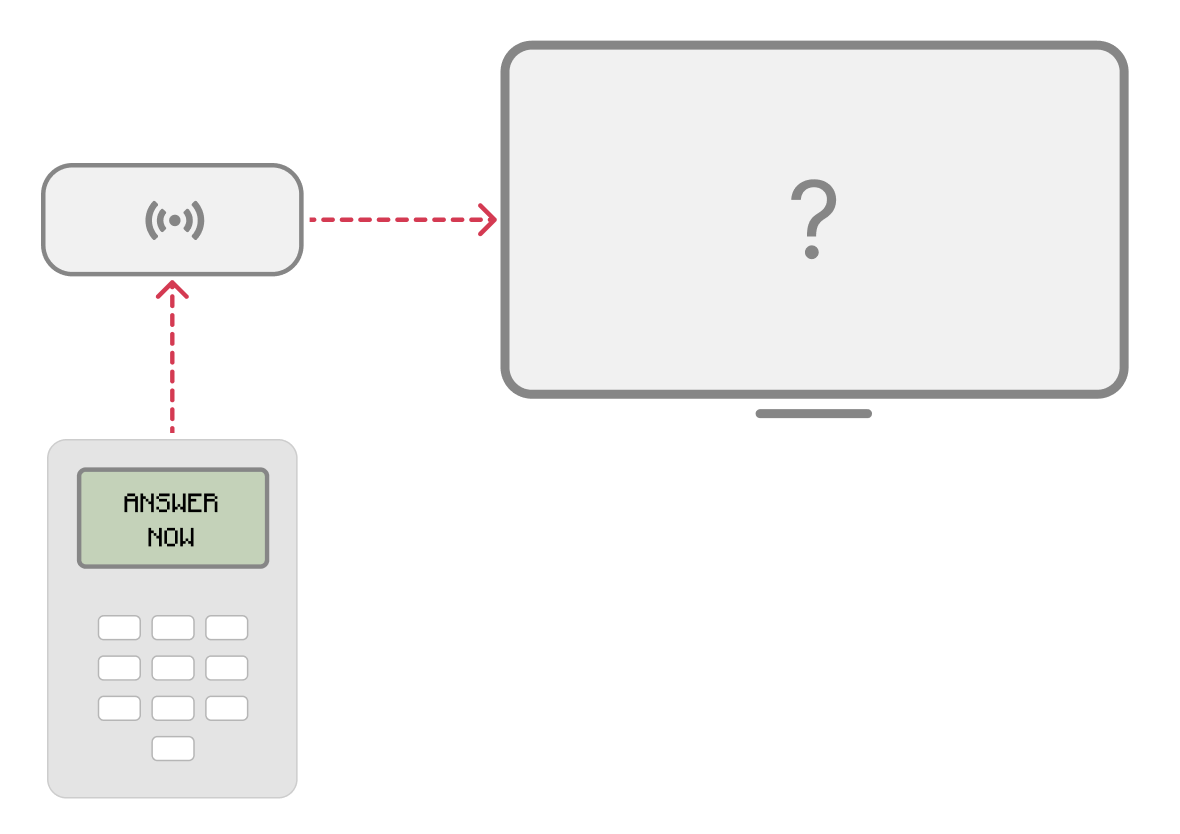
\includegraphics[width=1\linewidth]{figures/clickers-illustration.png}
    \caption{A typical classroom setup with clickers, a receiver and a tv}
    \label{fig:A typical classroom setup with clickers, a receiver and a tv}
\end{figure}


\subsection{Kahoot!}
Kahoot! is a software company that offers a digital solution where students use their mobile phone or computer as the tool for submitting answers.

This approach allows users to join sessions with their custom name and avatar, allowing a more individual approach. On top of this are features like music, leaderboard and scores tools used to further increase the engagement.

By utlizing the internet, the issues with infrared signals are solved, at the cost of requiring a stable internet connection. By utilizing existing hardware (assuming everyone has their own mobile phone), we can drastically reduce the cost of operations for the schools, enabling a more widespread usage. This approach also allows for participating remotely, making participation from digital classrooms and MOOCs possible as well. 

\todo{also mention about open-text grouping}

\begin{figure}[h!]
    \centering
    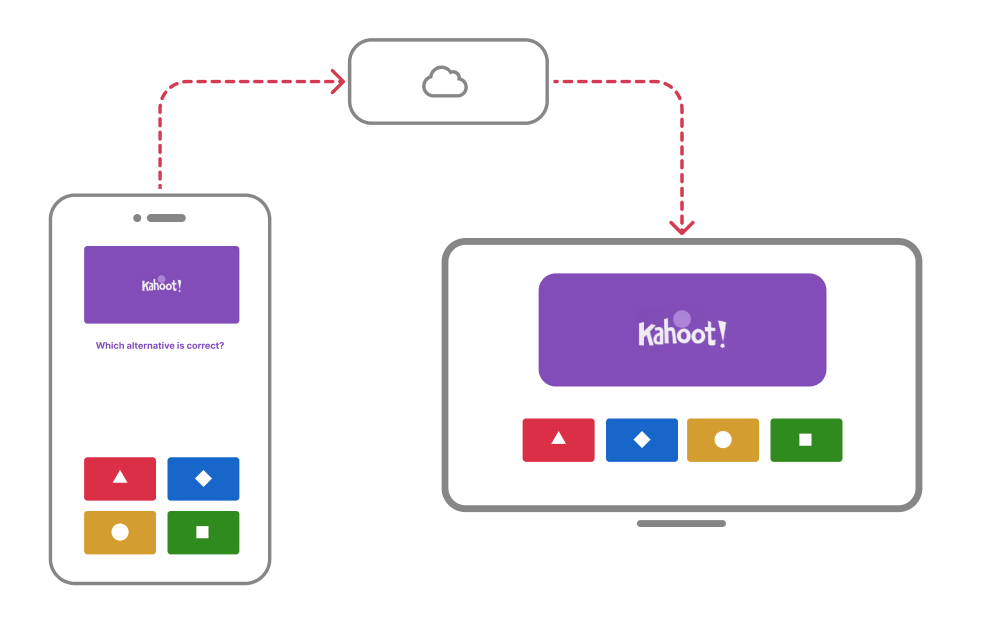
\includegraphics[width=1\linewidth]{figures/kahoot-illustration.png}
    \caption{A Kahoot setup with phones and a tv}
    \label{fig:kahoot}
\end{figure}

\subsection{Mentimeter}
% similar to Kahoot, word-clouds, polls
Mentimeter utilizes similar technology as Kahoot!. It leverages the personal device to connect to a session. 

Mentimeter differs in terms of use context. It has less focus on the gamification, and offers tools like word-clouds and polls.

The polls allow students to vote on different options, and then the graph of distributions will be shown on the screen, allowing students to compare answers. It also has support for other graphs like 1-5 (waves).

Mentimeter also allows users to submit open-text responses, which can be showcased in a word cloud
\todo{might also be able to visualize with boxes? (need to check this out)}
\todo{include images of the actual offering?}

\subsection{Live-questions (traditional)}
% not worth mentioning?
% Can be raise-of-hands as well? 

We have mostly focused on digital solutions, but it can be nice to get an overview of non-digital alternatives.

Raise-of-hands allow the lecturer to ask a question and cast a vote. This can either be yes/no, multiple-choice questions. While this is easy to implement, getting exact measures of distributions might be difficult. In digital classrooms, it might be difficult to get an overview if respondends have low camera quality or poor connection. In large lecture halls it might not be possible to see everyone present from the perspective of the lecturer. 

\section{Challenges with the current systems}
% Move to Discussion part
\todo{Move to discussion part}
% backbround should simply be information that people need to know before reading the thesis

\section{Problem of interpreting open-ended questions}
\todo{Large classrooms, actionable insights}
Interpreting written open-ended answers becomes more cumbersome based on the amount of responses. This usually means that such a system is difficult to use for large classes. 

The time it would take for the lecturer to read and comprehend the responses would take too much focus away from the lecture, potentially reducing the efficiency of the lecture. 

A possible solution could be to have a new role, responsible as administrator of the responses, which role is to read and make optimizations for the lecturer while the lecturer is teaching. However this might cause a weird dynamic, as processes in parallell might take focus away from the learning process.

While smaller classes might make it feasible to read through all responses, it might still be difficult to compare or group responses and make actionable insights. 

\section{Techniques: Promising topics for exploration: Text mining/AI}
\todo{Feature extration, topic modeling, topic extraction, summarization, AI}
% Can simply explain the different methods here
\todo{How computers can help make sense of unstructured text}

\section{Previous work in theory modules (IT3023)}
In the theory module (course-id IT3023) we explored and investigated the domain of educational data analysis and dashboard design, with the goal of enhancing student engagement and performance. The primary focus was related to a dataset that monitored the usage of an educational dashboard in the context of performing a course related quiz. Our data analysis revealed that increased usage of dashboard was correlated to better academic scores. The dataset also contained information on question difficulty, and we could determine that all kinds of questions benefited, even though the most difficult questions had slightly more improvement.

Building on these findings, we developed a prototype of a new educational dashbord solution in Figma. Since dashboard usage was a major factor in educational performance, we desiged the prototype with a goal of making the user want to use the dashboard more. We made sure that metrics like progress-tracking, accuracy and time-management were cleaarly visible, so that the user could become aware of, and also see progress. Our hypothesis is that being able to see your own progress would make it more motivating to use, and thus increasing student performance. The dashboard also incorporated features to make performance feedback more actionable, aligning with principles of gamification and metacognitive feedback.

\section{Plans for prototype}
\section{Testing of prototype}

% Explain AI, NLP, Text-mining, Sentimental Analysis

% Explain how this can extract themes, gauge sentiment, or detect common misconceptions

% Describe challenges of applying NLP to educational data, such as dealing with informal language, typos, or multilingual responses


\section{Positive impacts of our proposed system}

% Illustrate how AI-driven insights could influence lesson planning or live lecture adjustments, offering concrete examples like identifying misunderstood topics or gaps in student comprehension.

% Discuss how summarization or clustering could help lecturers prioritize feedback on students’ misunderstandings and adapt teaching in real-time.









\begin{comment}
Research projects should always be based on previous research on the same and/or related topics. This should be described as a background to the thesis with adequate bibliographical references. If the material needed is too voluminous to fit nicely in the review part of the introduction, it can be presented in a separate background chapter.
\end{comment}